%
% ---------------------------------------------------------------
% Copyright (C) 2012-2018 Gang Li
% ---------------------------------------------------------------
%
% This work is the default powerdot-tuliplab style test file and may be
% distributed and/or modified under the conditions of the LaTeX Project Public
% License, either version 1.3 of this license or (at your option) any later
% version. The latest version of this license is in
% http://www.latex-project.org/lppl.txt and version 1.3 or later is part of all
% distributions of LaTeX version 2003/12/01 or later.
%
% This work has the LPPL maintenance status "maintained".
%
% This Current Maintainer of this work is Gang Li.
%
%

\documentclass[
 size=14pt,
 paper=smartboard,  %a4paper, smartboard, screen
 mode=present, 		%present, handout, print
 display=slides, 	% slidesnotes, notes, slides
 style=tuliplab,  	% TULIP Lab style
 pauseslide,
 fleqn,leqno]{powerdot}


\usepackage{cancel}
\usepackage{caption}
\usepackage{stackengine}
\usepackage{smartdiagram}
\usepackage{attrib}
\usepackage{amssymb}
\usepackage{amsmath}
\usepackage{amsthm}
\usepackage{mathtools}
\usepackage{rotating}
\usepackage{graphicx}
\usepackage{boxedminipage}
\usepackage{rotate}
\usepackage{calc}
\usepackage[absolute]{textpos}
\usepackage{psfrag,overpic}
\usepackage{fouriernc}
\usepackage{pstricks,pst-3d,pst-grad,pstricks-add,pst-text,pst-node,pst-tree}
\usepackage{moreverb,epsfig,subfigure}
\usepackage{color}
\usepackage{booktabs}
\usepackage{etex}
\usepackage{breqn}
\usepackage{multirow}
\usepackage{natbib}
\usepackage{bibentry}
\usepackage{gitinfo2}
\usepackage{siunitx}
\usepackage{nicefrac}
%\usepackage{geometry}
%\geometry{verbose,letterpaper}
\usepackage{media9}
\usepackage{animate}
%\usepackage{movie15}
\usepackage{auto-pst-pdf}

\usepackage{breakurl}
\usepackage{fontawesome}
\usepackage{xcolor}
\usepackage{multicol}



\usepackage{verbatim}
\usepackage[utf8]{inputenc}
\usepackage{dtk-logos}
\usepackage{tikz}
\usepackage{adigraph}
%\usepackage{tkz-graph}
\usepackage{hyperref}
%\usepackage{ulem}
\usepackage{pgfplots}
\usepackage{verbatim}
\usepackage{fontawesome}


\usepackage{todonotes}
% \usepackage{pst-rel-points}
\usepackage{animate}
\usepackage{fontawesome}

\usepackage{listings}
\lstset{frameround=fttt,
frame=trBL,
stringstyle=\ttfamily,
backgroundcolor=\color{yellow!20},
basicstyle=\footnotesize\ttfamily}
\lstnewenvironment{code}{
\lstset{frame=single,escapeinside=`',
backgroundcolor=\color{yellow!20},
basicstyle=\footnotesize\ttfamily}
}{}


\usepackage{hyperref}
\hypersetup{ % TODO: PDF meta Data
  pdftitle={Presentation Title},
  pdfauthor={Gang Li},
  pdfpagemode={FullScreen},
  pdfborder={0 0 0}
}


% \usepackage{auto-pst-pdf}
% package to show source code

\definecolor{LightGray}{rgb}{0.9,0.9,0.9}
\newlength{\pixel}\setlength\pixel{0.000714285714\slidewidth}
\setlength{\TPHorizModule}{\slidewidth}
\setlength{\TPVertModule}{\slideheight}
\newcommand\highlight[1]{\fbox{#1}}
\newcommand\icite[1]{{\footnotesize [#1]}}

\newcommand\twotonebox[2]{\fcolorbox{pdcolor2}{pdcolor2}
{#1\vphantom{#2}}\fcolorbox{pdcolor2}{white}{#2\vphantom{#1}}}
\newcommand\twotoneboxo[2]{\fcolorbox{pdcolor2}{pdcolor2}
{#1}\fcolorbox{pdcolor2}{white}{#2}}
\newcommand\vpspace[1]{\vphantom{\vspace{#1}}}
\newcommand\hpspace[1]{\hphantom{\hspace{#1}}}
\newcommand\COMMENT[1]{}

\newcommand\placepos[3]{\hbox to\z@{\kern#1
        \raisebox{-#2}[\z@][\z@]{#3}\hss}\ignorespaces}

\renewcommand{\baselinestretch}{1.2}


\newcommand{\draftnote}[3]{
	\todo[author=#2,color=#1!30,size=\footnotesize]{\textsf{#3}}	}
% TODO: add yourself here:
%
\newcommand{\gangli}[1]{\draftnote{blue}{GLi:}{#1}}
\newcommand{\shaoni}[1]{\draftnote{green}{sn:}{#1}}
\newcommand{\gliMarker}
	{\todo[author=GLi,size=\tiny,inline,color=blue!40]
	{Gang Li has worked up to here.}}
\newcommand{\snMarker}
	{\todo[author=Sn,size=\tiny,inline,color=green!40]
	{Shaoni has worked up to here.}}

%%%%%%%%%%%%%%%%%%%%%%%%%%%%%%%%%%%%%%%%%%%%%%%%%%%%%%%%%%%%%%%%%%%%%%%%
% title
% TODO: Customize to your Own Title, Name, Address
%
\title{Flip 01 Project Report}
\author{
Jing Miao
\\
\\Qingdao University of Technology
}
\date{January 10th}


% Customize the setting of slides
\pdsetup{
% TODO: Customize the left footer, and right footer
rf=\href{http://www.tulip.org.au}{
Last Changed by: \textsc{\gitCommitterName}\ \gitVtagn-\gitAbbrevHash\ (\gitAuthorDate)
},
cf={Flip 01 Project Report},
}


\begin{document}

\maketitle

%\begin{slide}{Overview}
%\tableofcontents[content=sections]
%\end{slide}


%%==========================================================================================
%%
\begin{slide}[toc=,bm=]{Overview}
\tableofcontents[content=currentsection,type=1]
\end{slide}
%%
%%==========================================================================================


\section{Introduction}


%%==========================================================================================
%%
\begin{slide}{Project Introduction}
\begin{center}
\twotonebox{\rotatebox{90}{}}{\parbox{.86\textwidth}
{With all of the tweets circulating every second it is hard to tell whether the sentiment behind a specific tweet will impact a company,
or a person's, brand for being viral (positive),
or devastate profit because it strikes a negative tone.
Capturing sentiment in language is important in these times where decisions and reactions are created and updated in seconds.
The purpose of this task is to detect hate speech in tweets. For the sake of simplicity, if there is racist or sexist sentiment on Twitter, we will say that it contains hate speech. Therefore, the task is to classify racist or sexist tweets from other tweets.
If there is a system that can detect this type of text, it will definitely make the Internet and social media a better, non-malicious communication space.
}}
\end{center}
\end{slide}
%%
%%==========================================================================================
\section{Data Analysis}

%%==========================================================================================



\begin{slide}[toc=,bm=]{Statistical Analysis Data}
\begin{table}[tb]
\setlength{\abovecaptionskip}{0pt}
\setlength{\tabcolsep}{2pt}
\centering
\caption{The First Five Rows of The Train Data}
\scalebox{0.8}{
\begin{tabular}{c| c c c c }
\toprule
%\centering
   & \texttt{textID}  & \texttt{text} & \texttt{selected_text} & \texttt{sentiment} \\
\midrule
$0$
&  {$cb774db0d1$} &  {$ I`d have responded, if I were going $}
&  {$I`d have responded, if I were going$} &  {$neutral$}\\
$1$
&  {$549e992a42$} &  {$ Sooo SAD I will miss you here in San Diego!!! $}&
{$Sooo SAD$}&  {$negative$}\\
$2$
&  {$088c60f138$}	&  {$ my boss is bullying me... $}	
&  {$bullying me$}	&  {$negative$} \\
$3$
&  {$9642c003ef$}	&  {$ what interview! leave me alone $}	
&  {$leave me alone$}	&  {$negative$} \\
$4$
&  {$358bd9e861$}	&  {$ Sons of ****, why couldn`t they put them on t... $}	
&  {$Sons of ****,$}	&  {$negative$}\\
\bottomrule
\end{tabular}
}
\end{table}
\begin{table}[tb]
\setlength{\abovecaptionskip}{0pt}
\setlength{\tabcolsep}{2pt}
\centering
\caption{The First Five Rows of The Test Data}
\scalebox{0.8}{
\begin{tabular}{c| c c c  }
\toprule
%\centering
   & \texttt{textID}  & \texttt{text} & \texttt{sentiment} \\
\midrule
$0$
&  {$f87dea47db$} &  {$ Last session of the day http://twitpic.com/67ezh $}
&  {$neutral$}\\
$1$
&  {$96d74cb729$} &  {$ Shanghai is also really exciting (precisely -... $}
& {$positive$}\\
$2$
&  {$eee518ae67$}	&  {$ Recession hit Veronique Branquinho, she has to... $}	
&  {$negative$} \\
$3$
&  {$01082688c6$}	&  {$ happy bday! $}	
&  {$positive$} \\
$4$
&  {$33987a8ee5$}	&  {$ http://twitpic.com/4w75p - I like it!! $}	
&  {$positive$}\\
\bottomrule
\end{tabular}
}
\end{table}
\end{slide}

%%==========================================================================================

\begin{slide}[toc=,bm=]{Statistical Analysis Data}
\begin{table}[tb]
\setlength{\abovecaptionskip}{0pt}
\setlength{\belowcaptionskip}{10pt}
\centering
\caption{Train Data Describe}
\scalebox{0.9}{
\begin{tabular}{c| c c c c}
\toprule
%\centering
   & \texttt{textID}  & \texttt{text} & \texttt{selected_text} & \texttt{sentiment} \\
\midrule
$count$
&  {$27481$}	&  {$27480$}	&  {$27480$}	&  {$27481$}\\
$unique$
&  {$27481$}	&  {$27480$}	&  {$22463$}	&  {$3$}\\
$top$
&  {$703d8ea662$}	&  {$hiii im on my ipod...i cant fall asleep$}	&  {$good$}	&  {$neutral$}\\
$freq$	
&  {$1$}	&  {$1$}	&  {$199$}	&  {$11118$}\\
\bottomrule
\end{tabular}
}
\end{table}
\end{slide}
%%
%%==========================================================================================

%%==========================================================================================
%%==========================================================================================

\begin{slide}[toc=,bm=]{Data Visualization}
\begin{itemize}
\item
To draw a Funnel-Chart for better visualization
\end{itemize}
\vspace{-0.8cm}
\begin{center}
   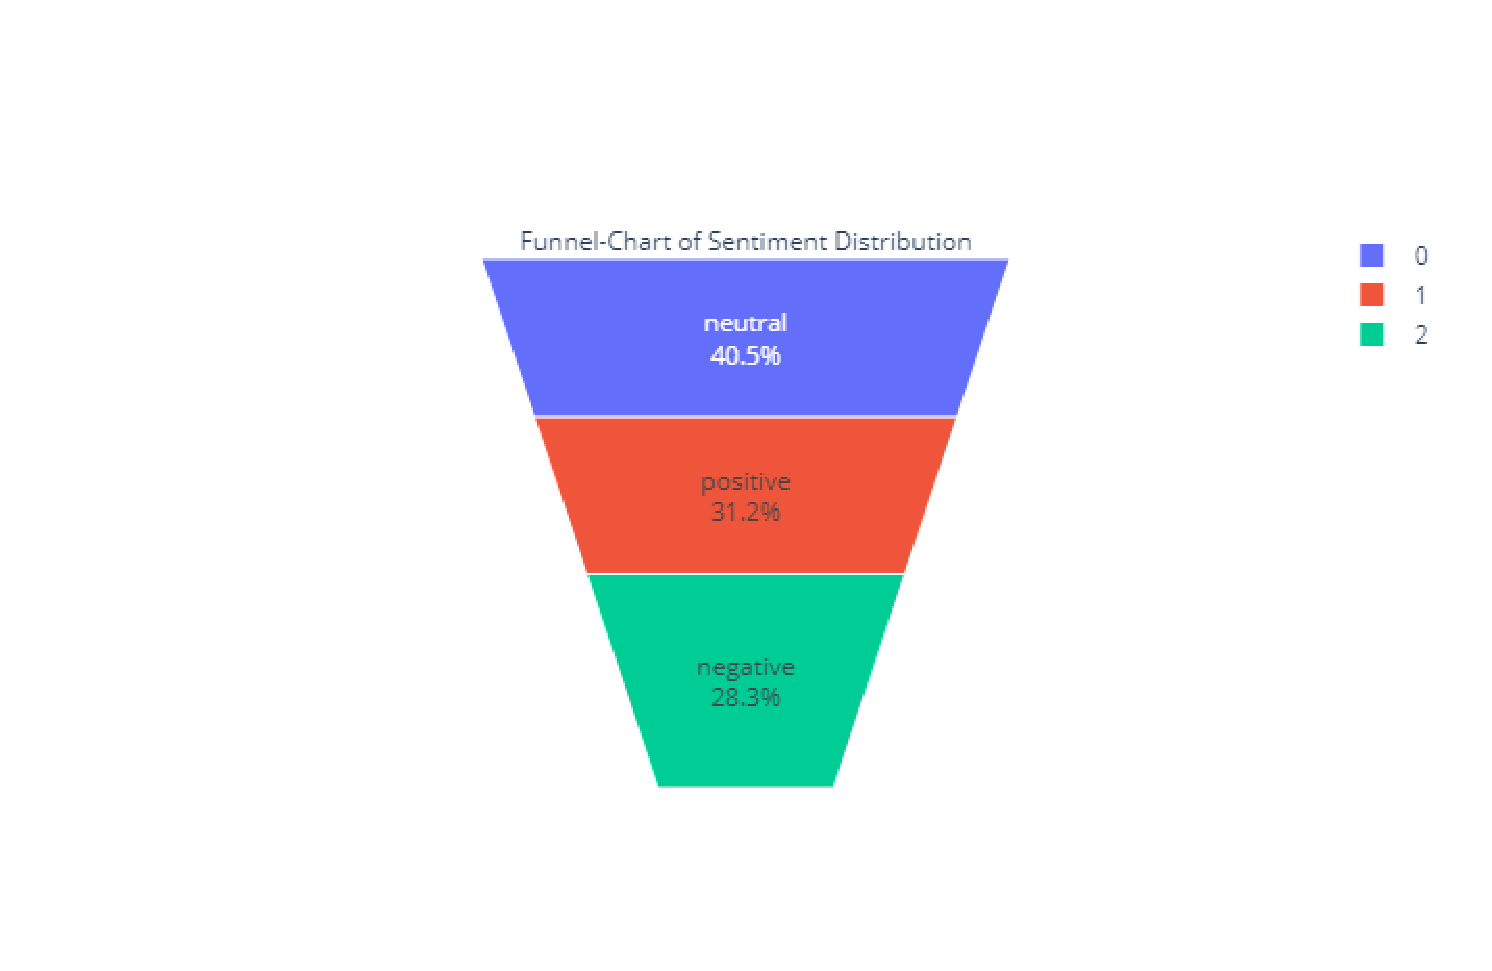
\includegraphics[width=.9\linewidth,height=.45\linewidth]{C:/FLIP01report/picture/newplot.eps}
\end{center}
\begin{itemize}
\item
From the above Funnel-Chart,the neutral sentiment accounted for the majority, followed by the positive and the least negative.
\end{itemize}
\end{slide}

%%==========================================================================================
\begin{slide}{Data Visualization}
\begin{itemize}
\item
So further analysis is needed to check the difference in Number of Words and the Jaccard Scores similarity across Different Sentiments between Text and selected_text.
\end{itemize}
\vspace{-0.8cm}
\begin{figure}[htbp]
\centering
\subfigure[Negative and Positive Sentiment]{
\begin{minipage}[t]{0.5\linewidth}
\centering
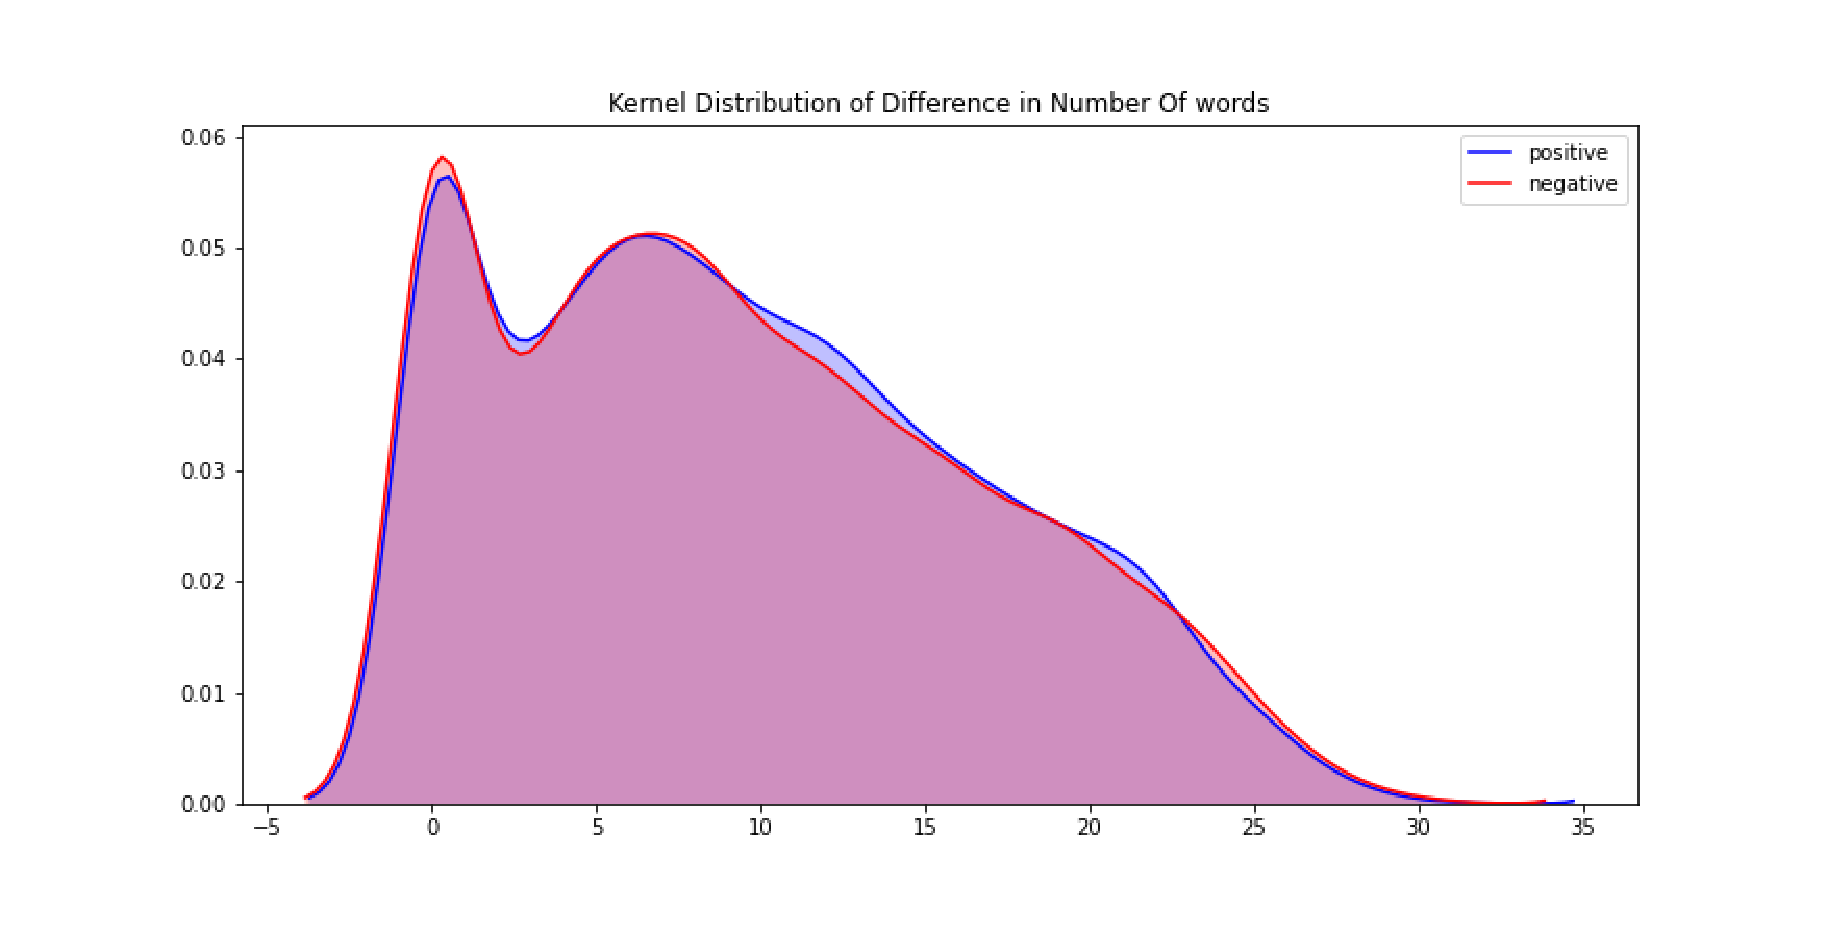
\includegraphics[width=3.5in, height=2.8in]{C:/FLIP01report/picture/difnum.eps}
%\caption{fig1}
\end{minipage}%
}%
\subfigure[Negative and Positive Sentiment]{
\begin{minipage}[t]{0.5\linewidth}
\centering
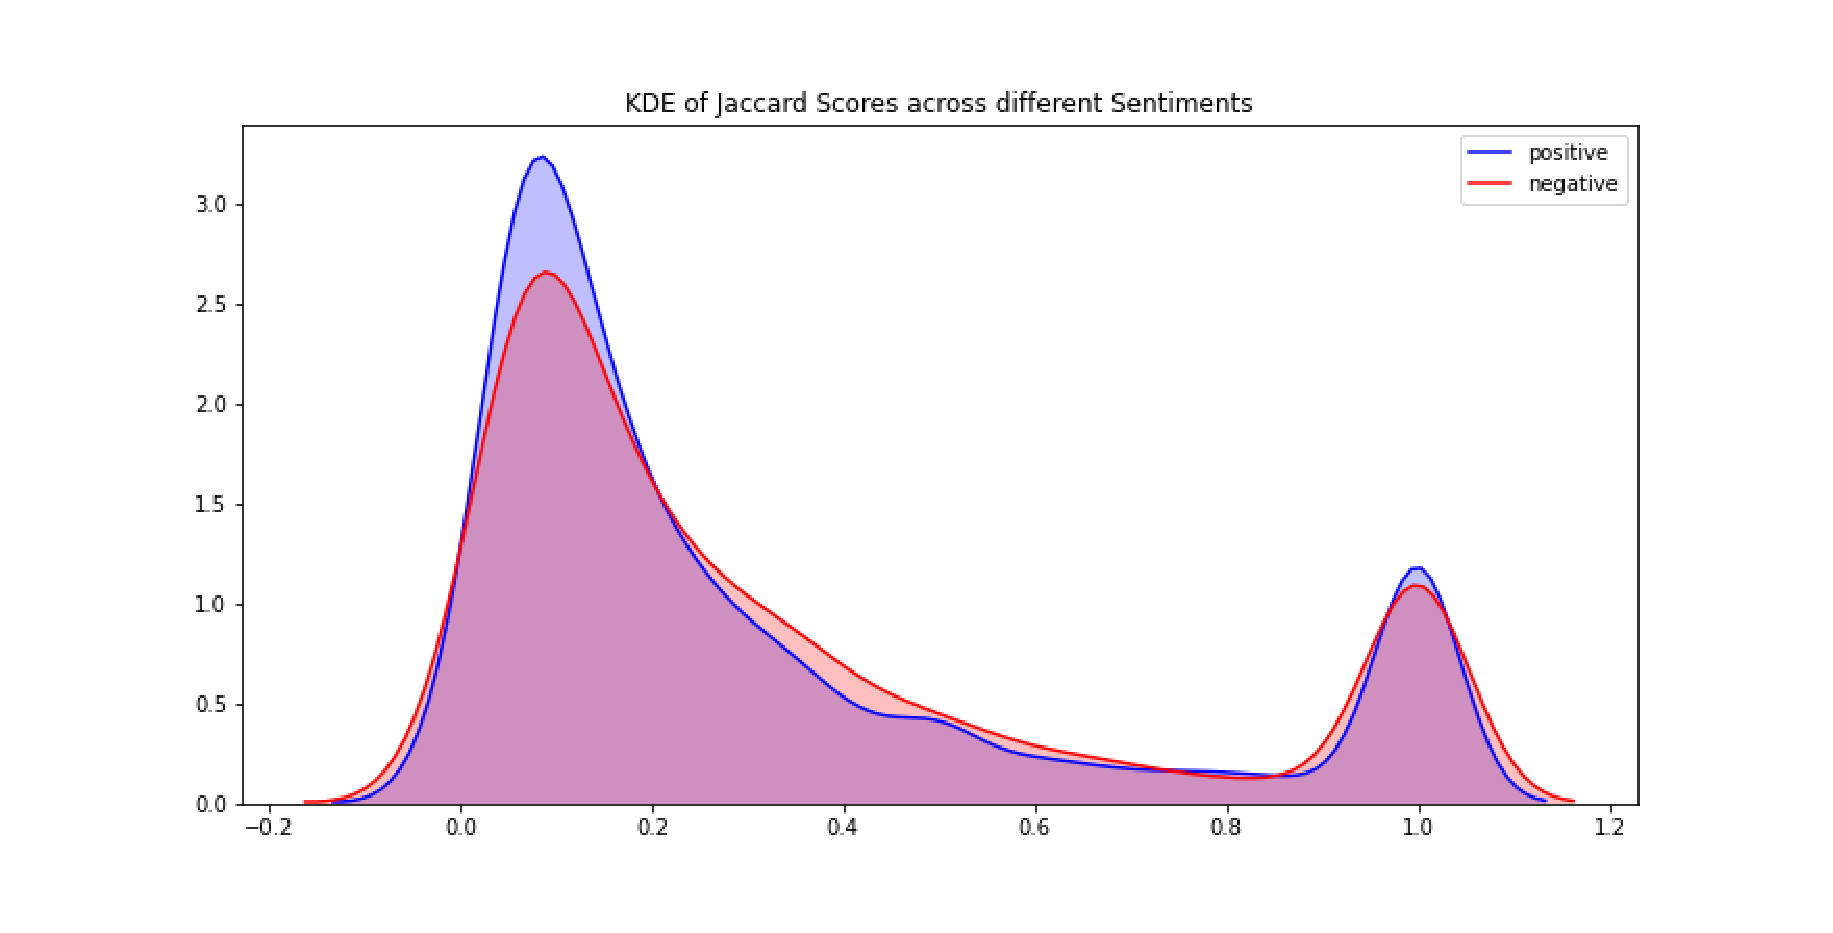
\includegraphics[width=3.5in, height=2.8in]{C:/FLIP01report/picture/jaccard1.eps}
%\caption{fig2}
\end{minipage}%
}%
\centering
\end{figure}
\end{slide}

%%==========================================================================================

\begin{slide}[toc=,bm=]{Data Visualization}
\vspace{-0.8cm}
\begin{figure}[htbp]
\centering
\subfigure[Difference in Number of Words in Neutral Sentiment]{
\begin{minipage}[t]{0.5\linewidth}
\centering
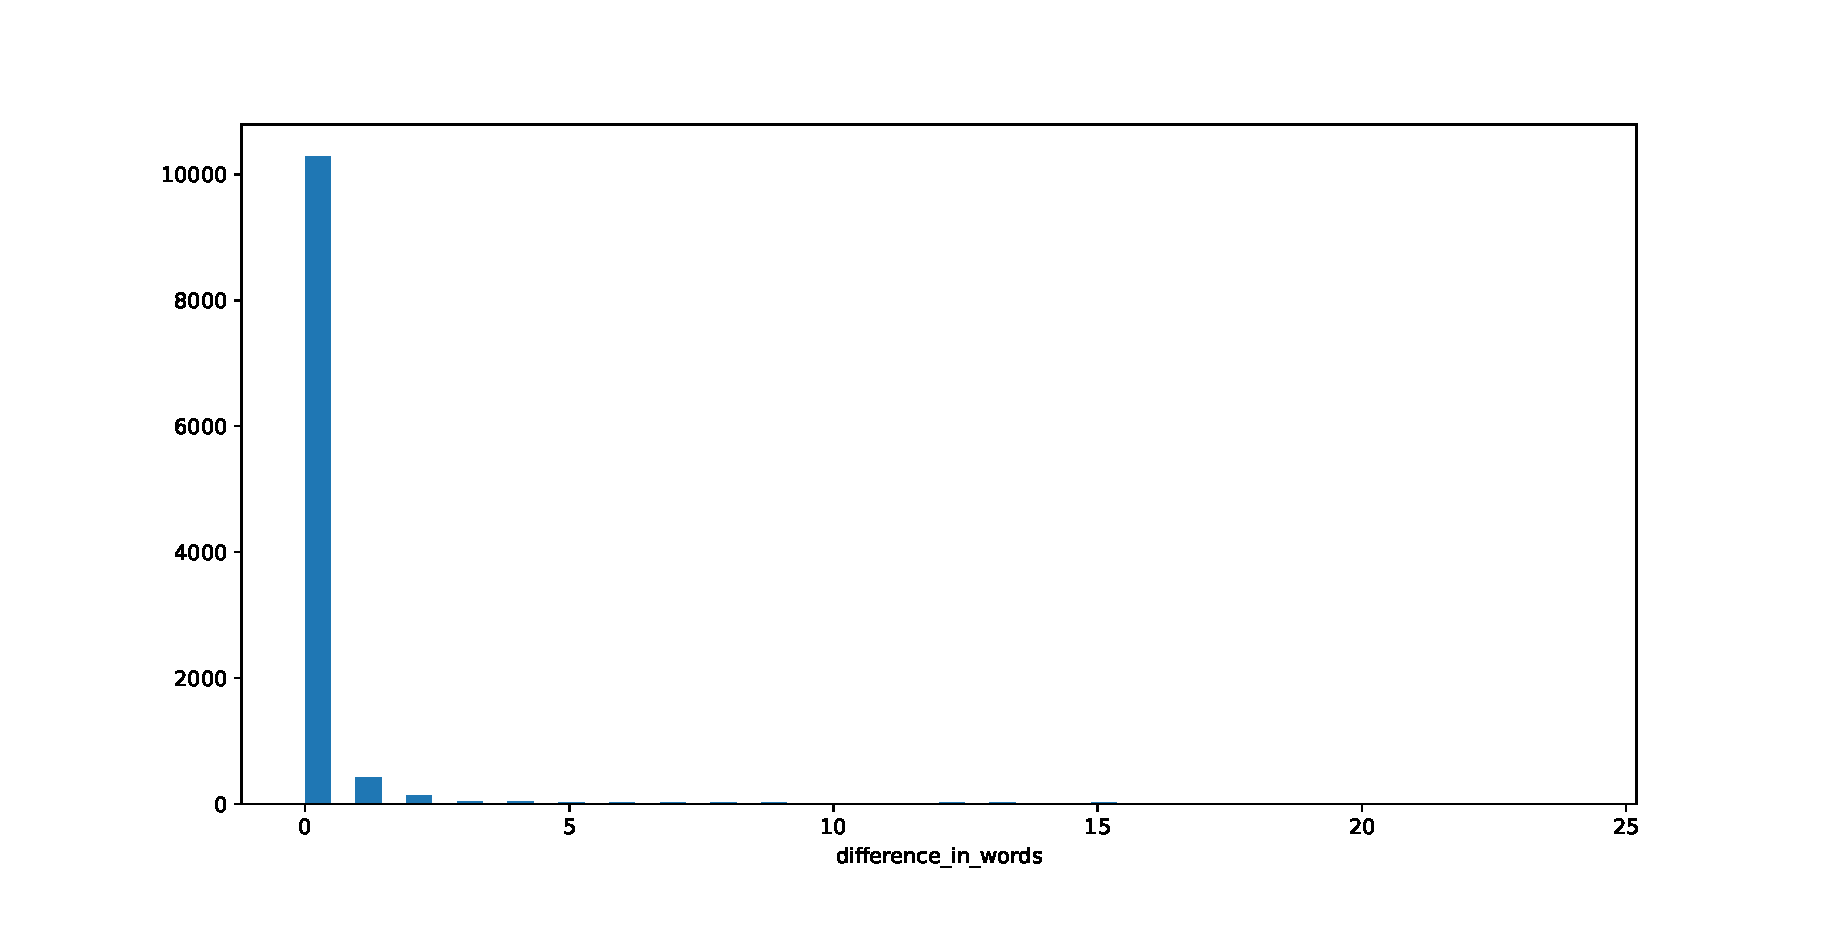
\includegraphics[width=3.5in, height=2.8in]{C:/FLIP01report/picture/difnumneu.eps}
%\caption{fig1}
\end{minipage}%
}%
\subfigure[Jaccard Scores in Neutral Sentiment]{
\begin{minipage}[t]{0.5\linewidth}
\centering
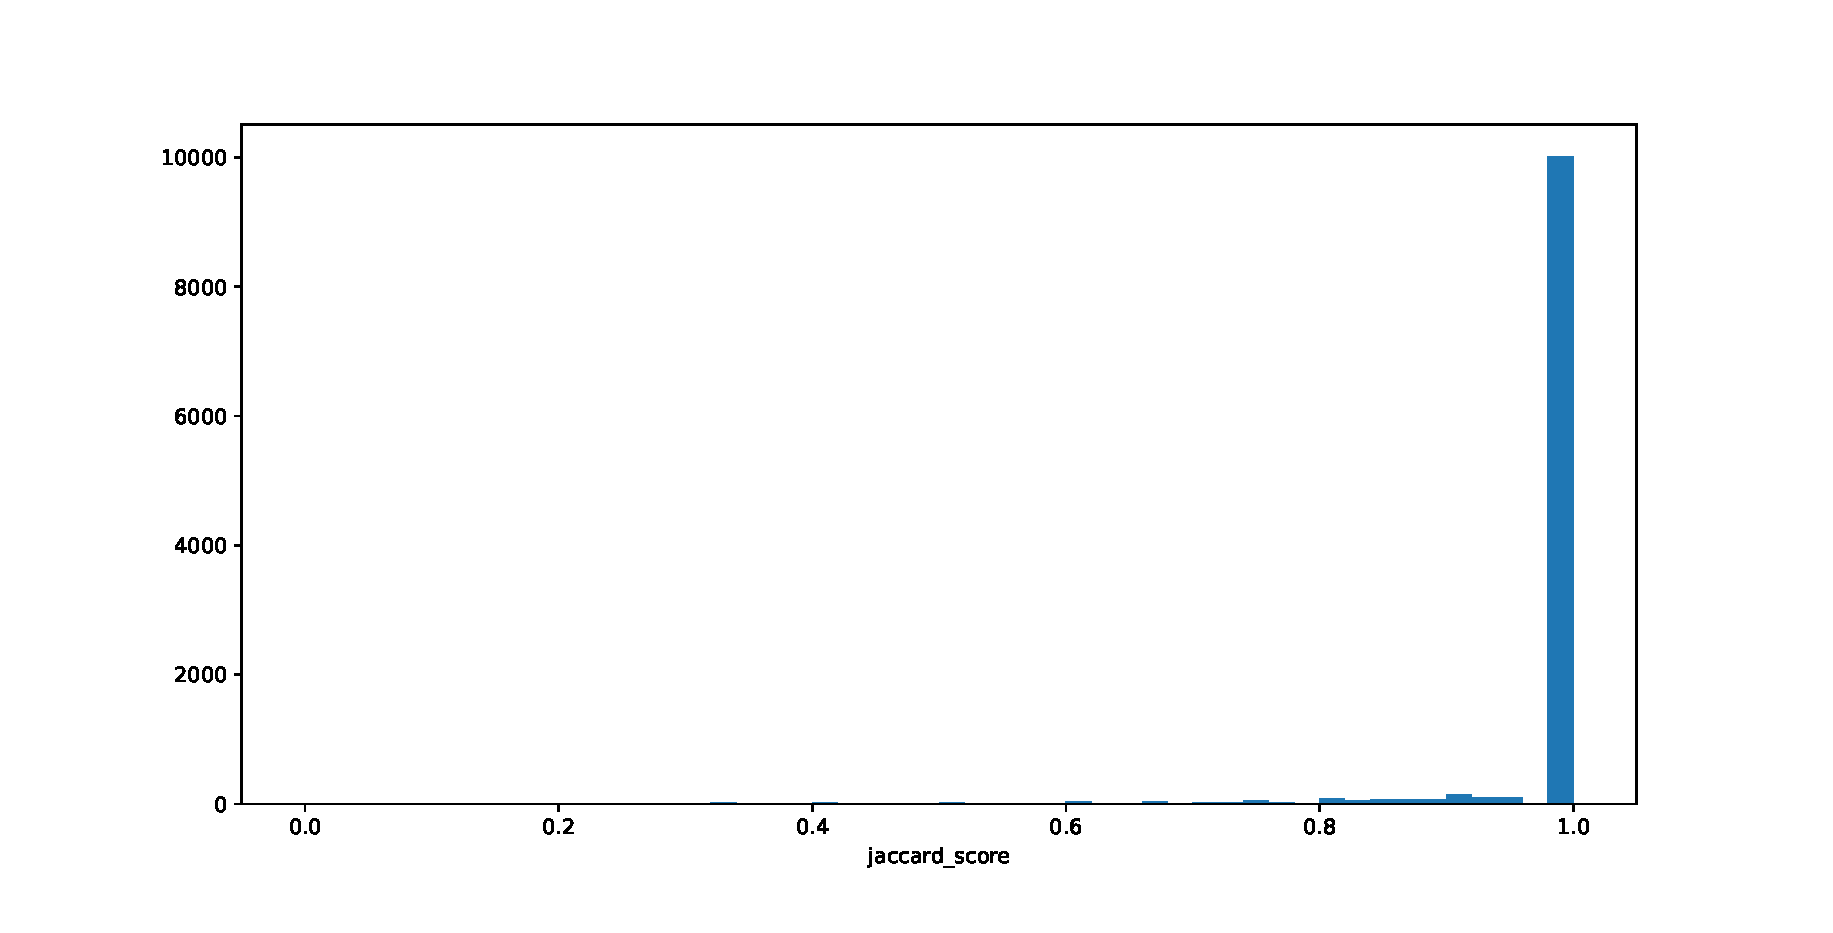
\includegraphics[width=3.5in, height=2.8in]{C:/FLIP01report/picture/jaccard2.eps}
%\caption{fig2}
\end{minipage}%
}%
\centering
\end{figure}
\end{slide}
%%==========================================================================================
%%==========================================================================================

\begin{slide}[toc=,bm=]{Conclusion Of EDA}
\begin{itemize}
\item
It can be seen that the number of tweets with a jaccard similarity of 1 between text extraction and text is more neutral sentiment.In conclusion maybe we can use neutral "text" as it is for "selected_text" in test data submission.
\item
We can see from the Jaccard Score Plot that there is peak for negative and positive plot around score of 1 .That means there is a cluster of tweets where there is a high similarity between text and selected texts ,if we can find those clusters then we can predict text for selected texts for those tweets irrespective of segment.
\end{itemize}
\end{slide}
%%==========================================================================================

\begin{slide}[toc=,bm=]{Data Visualization}
\begin{itemize}
\item
View the Jaccard value of positive tweets with words less than or equal to 2
\end{itemize}
\begin{center}
  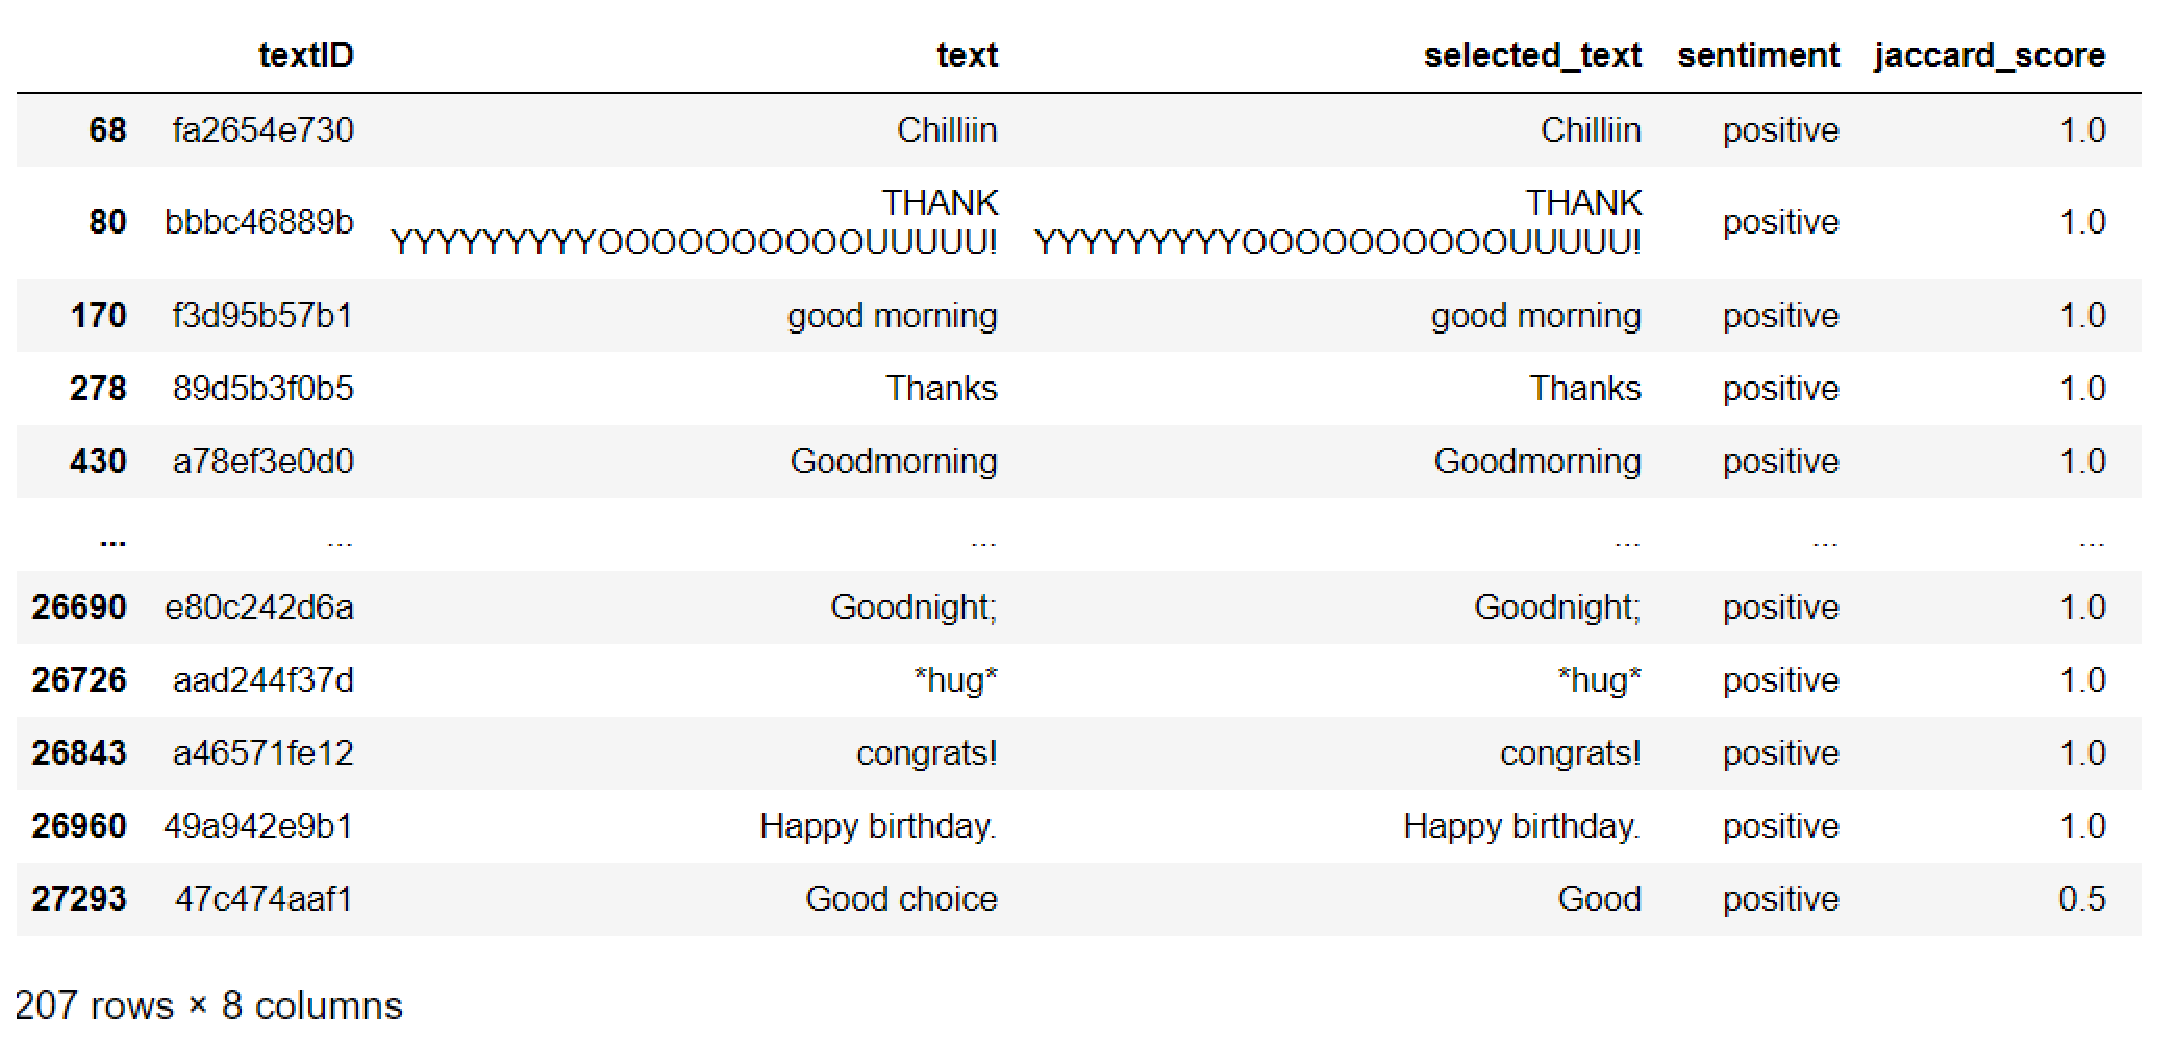
\includegraphics[width=.8\linewidth,height=.4\linewidth]{C:/FLIP01report/picture/jaccard3.eps}
\end{center}
\end{slide}
%%==========================================================================================

\section{Data cleaning}

%%==========================================================================================

\begin{slide}[toc=,bm=]{Data cleaning}
\begin{itemize}
\item
First,make text lowercase,remove text in square brackets,remove links,remove punctuation and remove words containing numbers.
\item
Then to remove the stopwords.
\end{itemize}
\end{slide}

%%==========================================================================================

%%==========================================================================================

\begin{slide}[toc=,bm=]{Data cleaning}
\begin{itemize}
\item
We can see that the top 20 most common words and the text in the selected text are almost the same.
\end{itemize}
\vspace{-0.8cm}
\begin{figure}[htbp]
\centering
\subfigure[]{
\begin{minipage}[t]{0.5\linewidth}
\centering
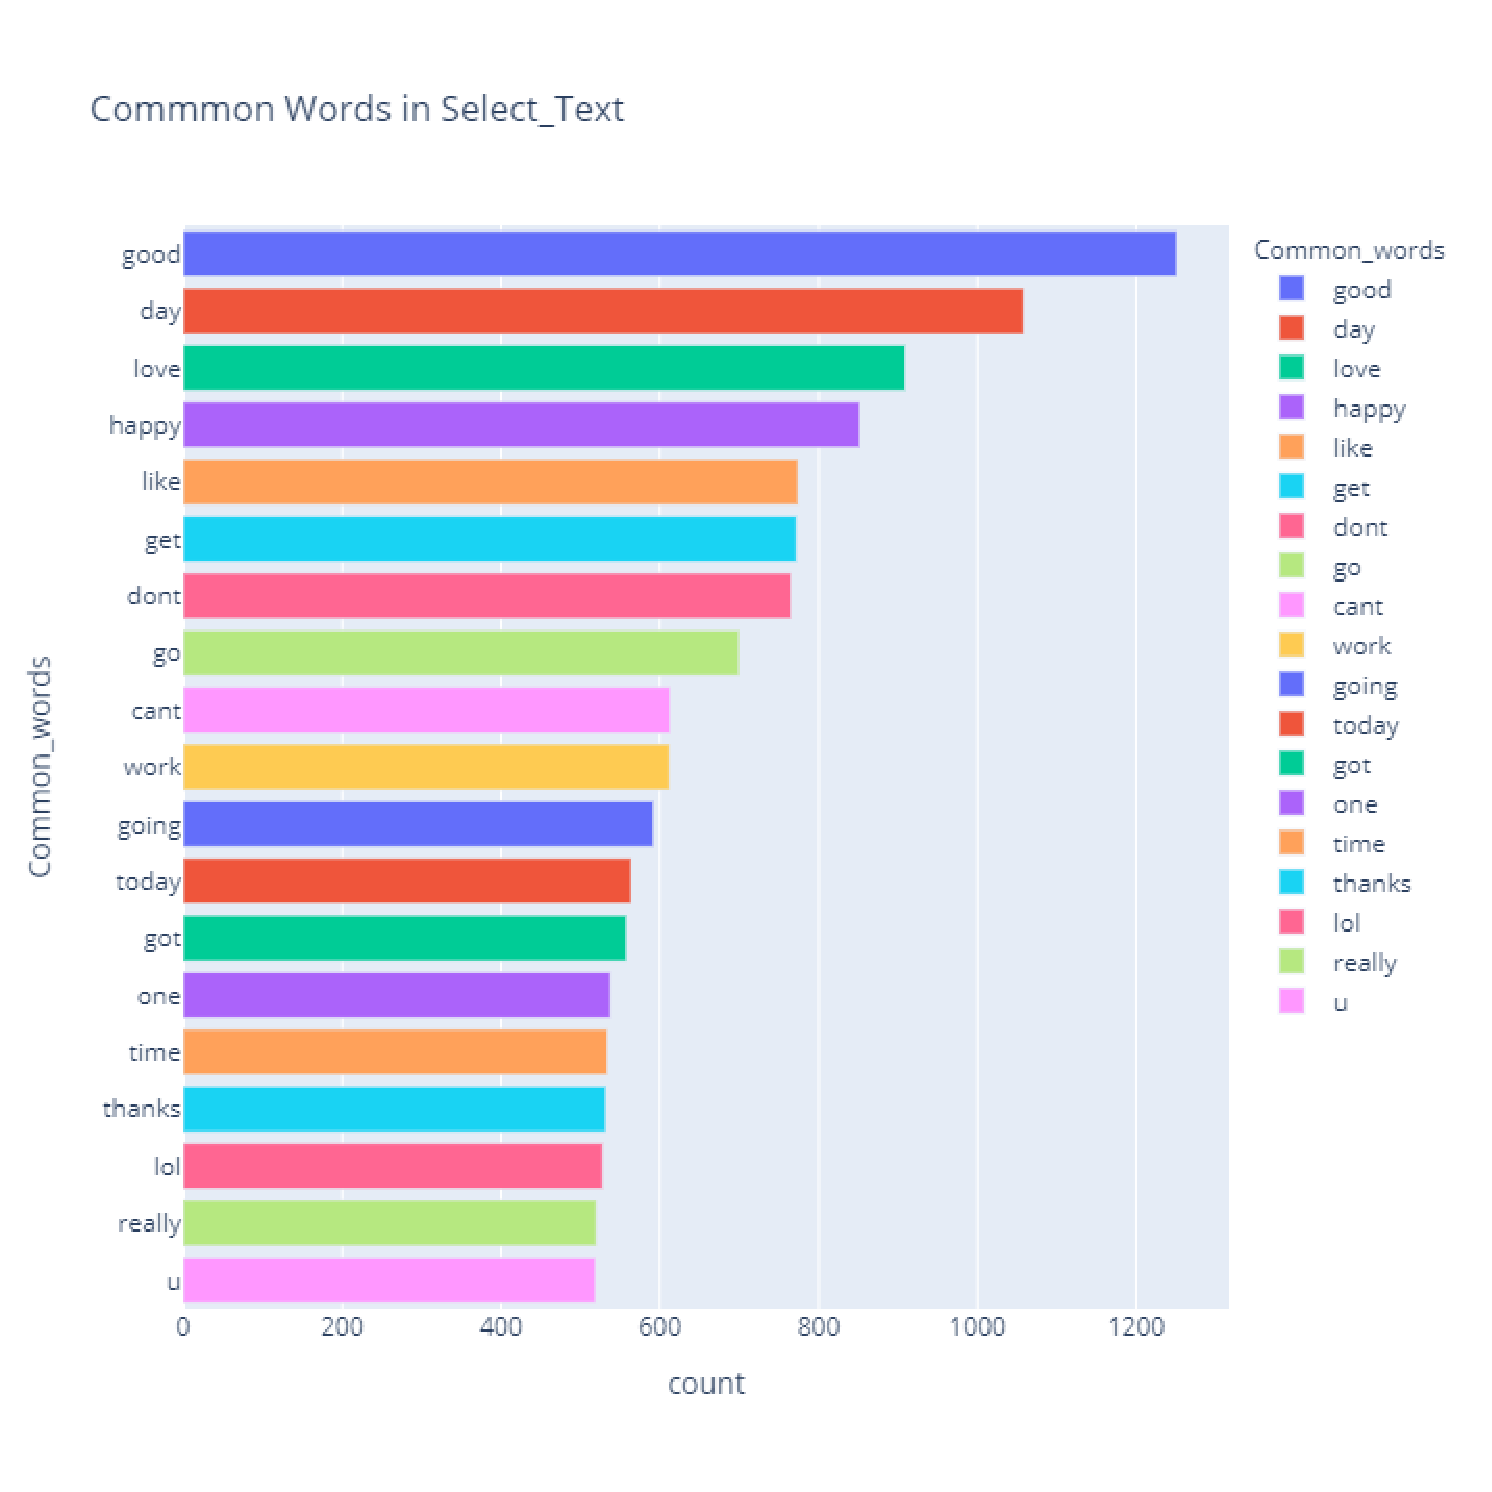
\includegraphics[width=3.5in, height=2.8in]{C:/FLIP01report/picture/com-stest-aft.eps}
%\caption{fig1}
\end{minipage}%
}%
\subfigure[]{
\begin{minipage}[t]{0.5\linewidth}
\centering
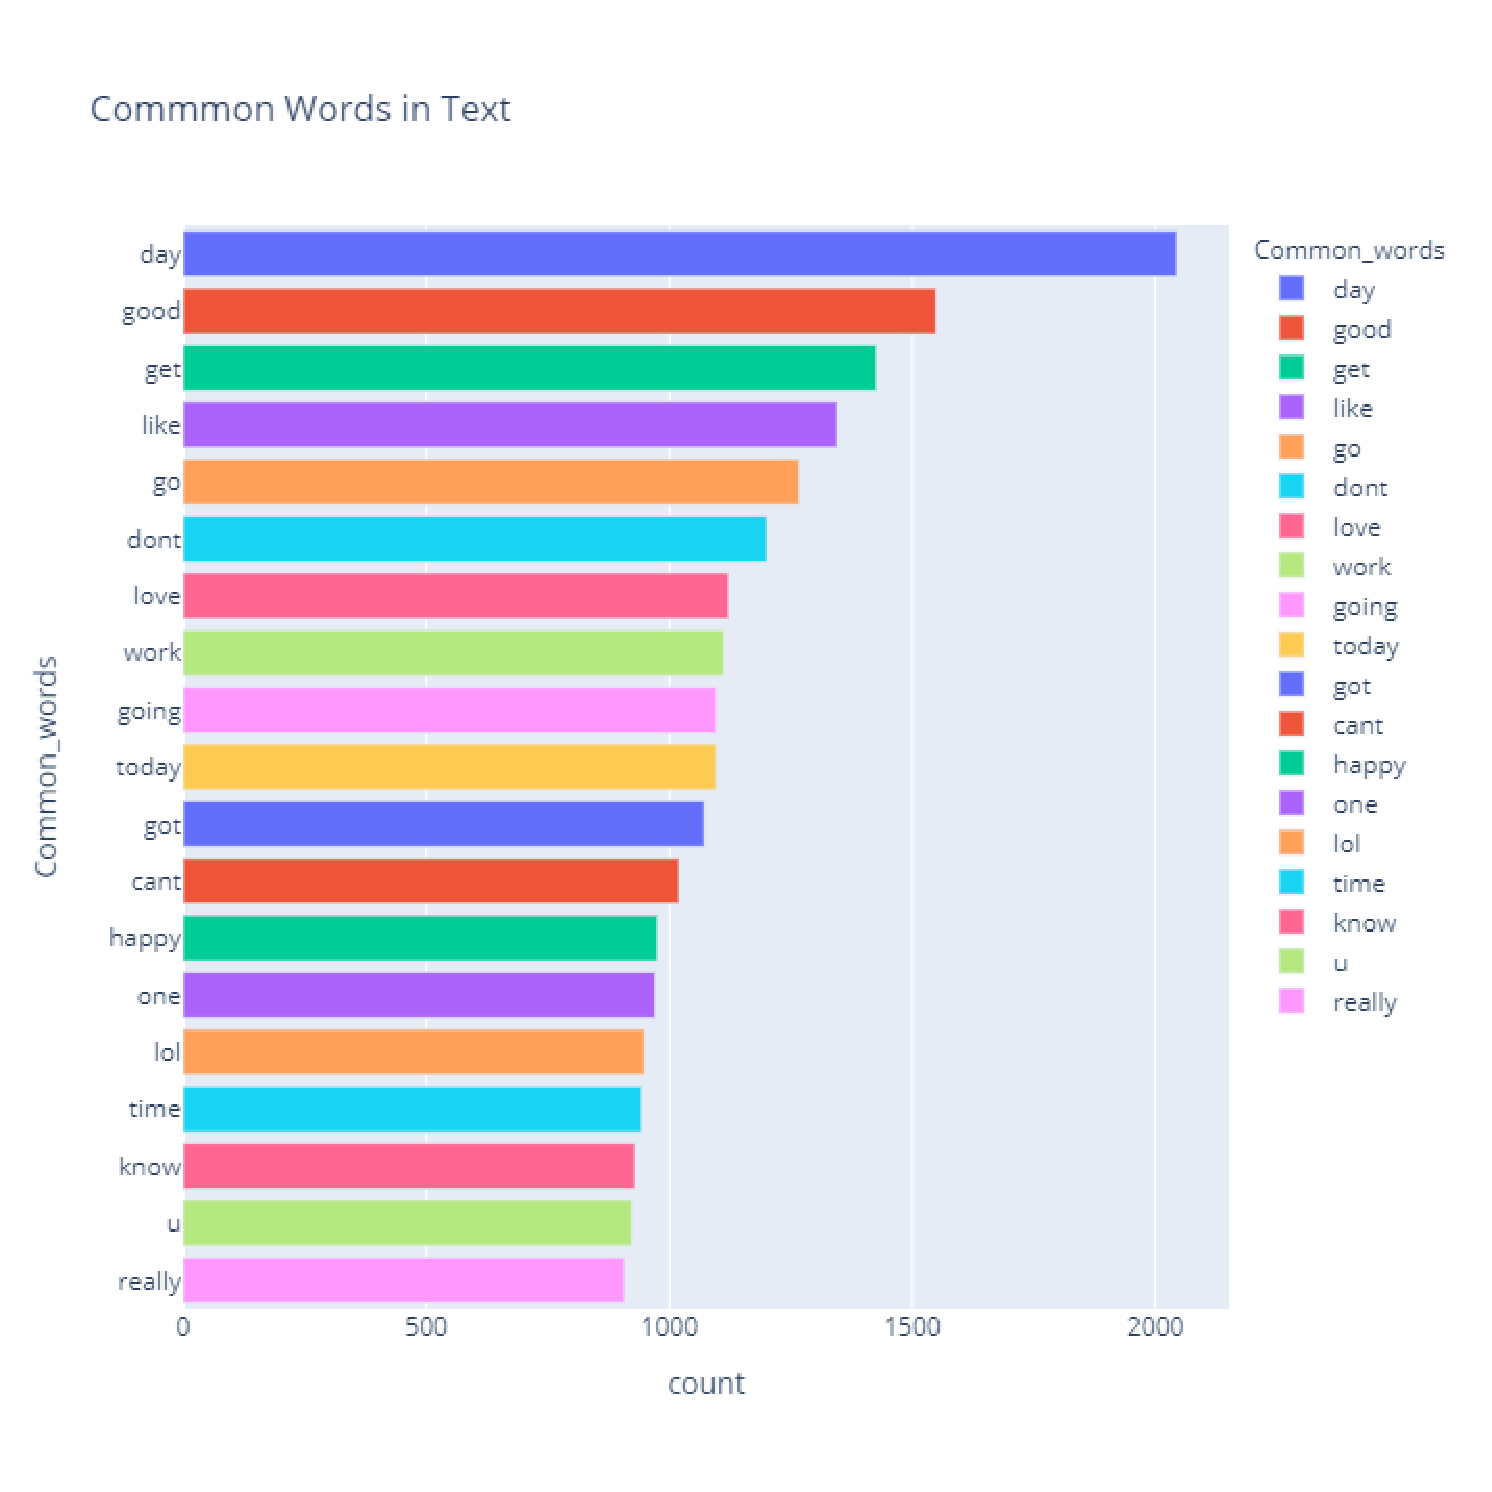
\includegraphics[width=3.5in, height=2.8in]{C:/FLIP01report/picture/com-test-aft.eps}
%\caption{fig2}
\end{minipage}%
}%
\centering
\end{figure}
\end{slide}

%%==========================================================================================
%%==========================================================================================
%%
\section{Data Feature Analysis}
%%==========================================================================================
%%
\begin{slide}[toc=,bm=]{Data Feature Analysis}
\begin{itemize}
\item
Unique Words in each Segment
\end{itemize}
\vspace{-0.8cm}
\begin{center}
  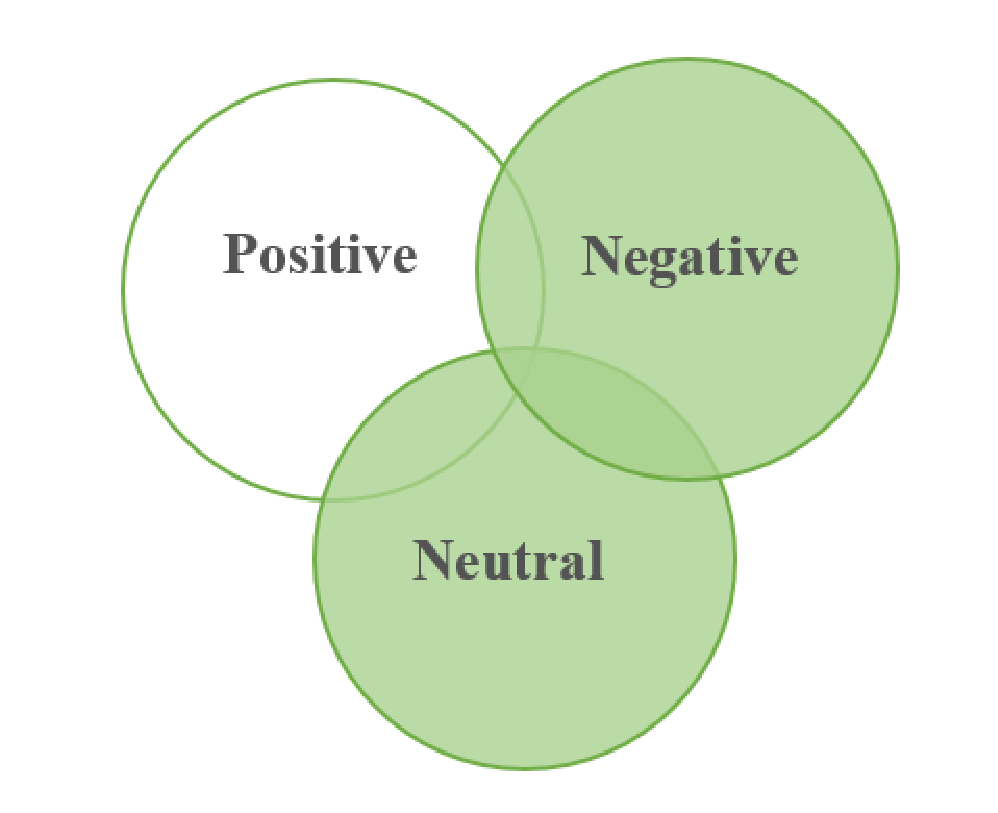
\includegraphics[width=.8\linewidth,height=.5\linewidth]{C:/FLIP01report/picture/unique.eps}
\end{center}
\end{slide}

%%==========================================================================================
%%==========================================================================================

\begin{slide}[toc=,bm=]{Data Feature Analysis}
\begin{itemize}
\item
Unique Words in each Segment
\item
By Looking at the Unique Words of each sentiment,we now have much more clarity about the data,these unique words are very strong determiners of Sentiment of tweets
\end{itemize}
\vspace{-0.8cm}
\begin{figure}[htbp]
\centering
\subfigure[Positive]{
\begin{minipage}[t]{0.3\linewidth}
\centering
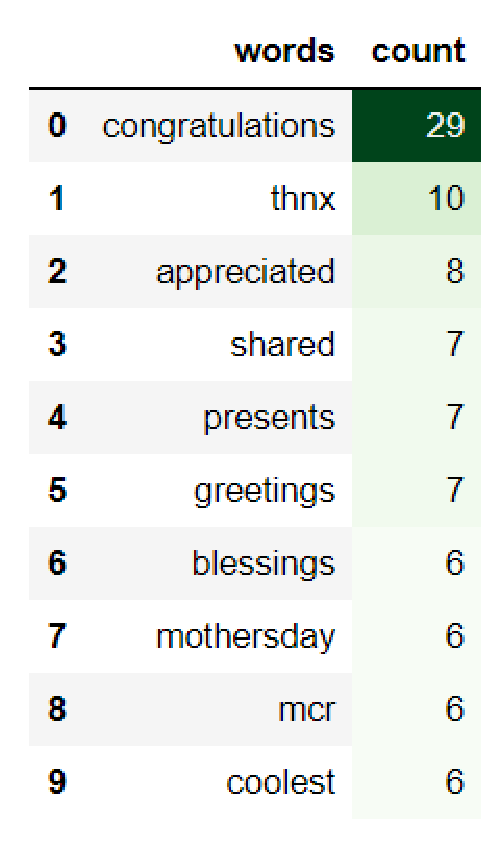
\includegraphics[width=1.8in, height=2.8in]{C:/FLIP01report/picture/unique-positive.eps}
%\caption{fig1}
\end{minipage}%
}%
\subfigure[Negative]{
\begin{minipage}[t]{0.3\linewidth}
\centering
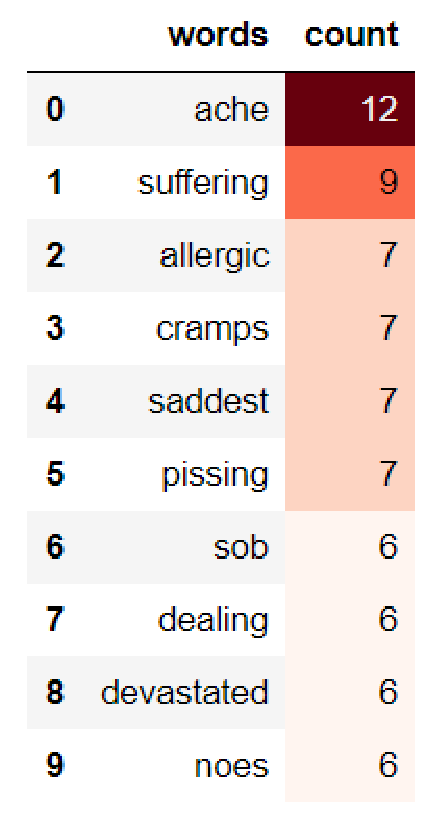
\includegraphics[width=1.8in, height=2.8in]{C:/FLIP01report/picture/unique-negative.eps}
%\caption{fig2}
\end{minipage}%
}%
\subfigure[Neutral]{
\begin{minipage}[t]{0.3\linewidth}
\centering
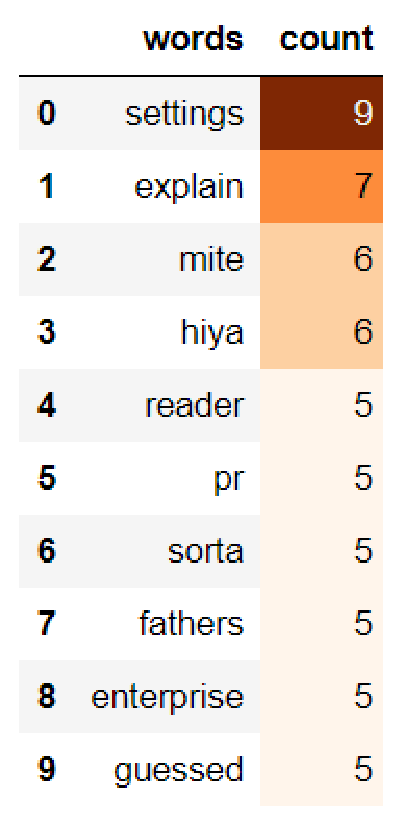
\includegraphics[width=1.8in, height=2.8in]{C:/FLIP01report/picture/unique-neutral.eps}
%\caption{fig2}
\end{minipage}
}%
\centering
\end{figure}
\end{slide}

%%=========================================================================================
%%==========================================================================================

\begin{slide}[toc=,bm=]{WordClouds}
\begin{itemize}
\item
Word Cloud of Negative Tweets
\end{itemize}
\vspace{-0.8cm}
\begin{center}
  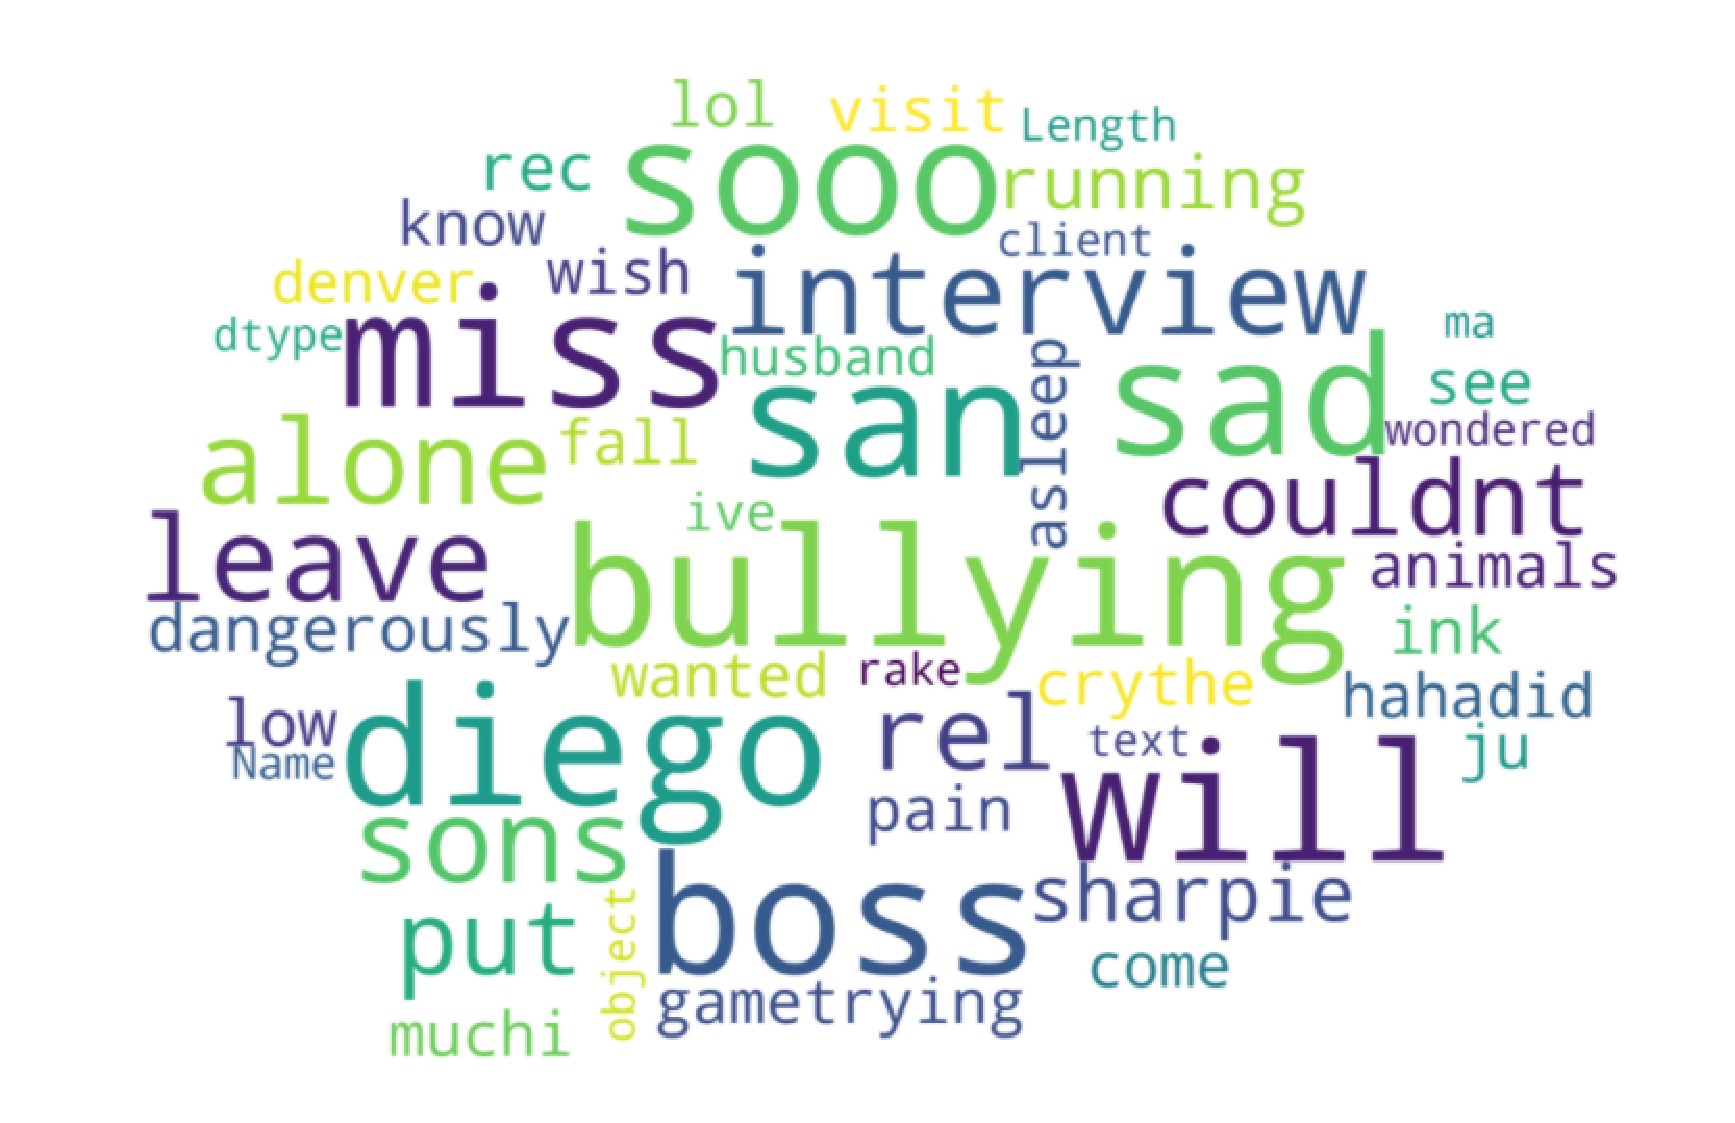
\includegraphics[width=.8\linewidth,height=.5\linewidth]{C:/FLIP01report/picture/Wcloud-neutral.eps}
\end{center}
\end{slide}

%%==========================================================================================
%%==========================================================================================
\section{Model}

%%==========================================================================================
%%==========================================================================================
\begin{slide}[toc=,bm=]{Model-NER}
\begin{itemize}
\item
To use text as selected_text for all neutral tweets due to their high jaccard similarity.
\item
To use text as selected_text for all tweets having number of words less than 3 in text.
\item
Train two different models for Positive and Negtive tweets.
\item
To use spacy for creating our own customised NER model or models (seperate for each Sentiment).
\end{itemize}
\end{slide}
%%==========================================================================================
%%==========================================================================================
%%=========================================================================================

\begin{slide}[toc=,bm=]{Train Model-NER}
\begin{itemize}
\item
Set up the pipeline and train the entity recognizer,create the built-in pipeline components and add them to the pipeline
\item
Add labels: entities
\item
get names of other pipes to disable them during training
\item
The sample can be divided into equal subsets, one gradient descent can be made for each subset, then the values of parameters W and B can be updated, and then the gradient descent can be continued in the next subset.
\item
Training models for Positive and Negative tweets.
\end{itemize}
\end{slide}
%%=========================================================================================
\begin{slide}[toc=,bm=]{Test Model-NER}
\begin{itemize}
\item
Unique Words in each Segment
\end{itemize}
\vspace{-0.8cm}
\begin{figure}[htbp]
\centering
\subfigure[]{
\begin{minipage}[t]{0.5\linewidth}
\centering
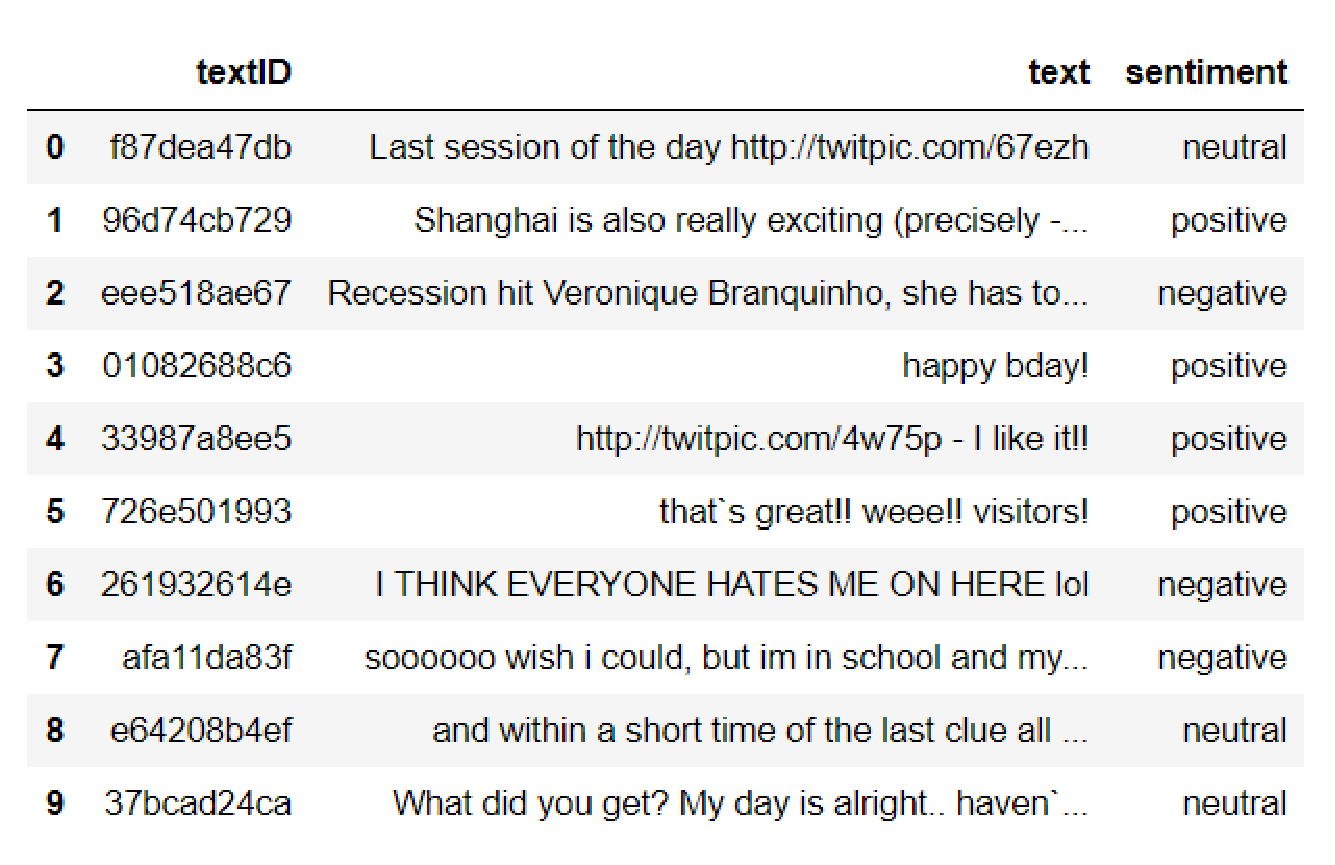
\includegraphics[width=3.3in, height=2.8in]{C:/FLIP01report/picture/test-pre.eps}
%\caption{fig1}
\end{minipage}%
}%
\subfigure[]{
\begin{minipage}[t]{0.5\linewidth}
\centering
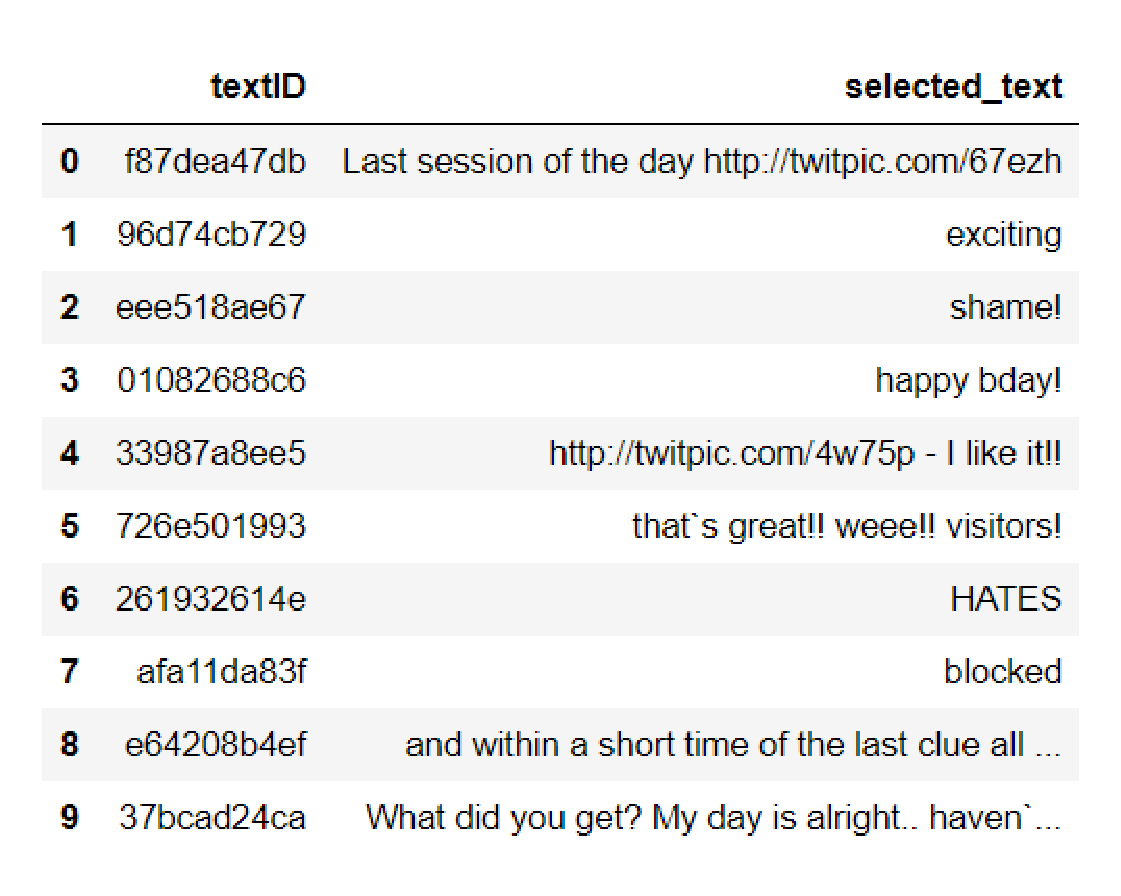
\includegraphics[width=3.5in, height=2.8in]{C:/FLIP01report/picture/test.eps}
%\caption{fig2}
\end{minipage}%
}%
\centering
\end{figure}
\end{slide}

%%=========================================================================================
%%=========================================================================================

\begin{slide}[toc=,bm=]{Model-BERT}
\begin{itemize}
\item
Data analysis, data visualization and data cleaning are all consistent with the above. Bert model is used for prediction, and the accuracy of this model is higher than that of NER model Z in natural language processing.
\end{itemize}
\end{slide}

%%=========================================================================================
%%=========================================================================================


\begin{slide}[toc=,bm=]{Train Model-BERT}
\begin{itemize}
\item
The Jaccard socre of training iteration 5 times.
\end{itemize}
\begin{center}
  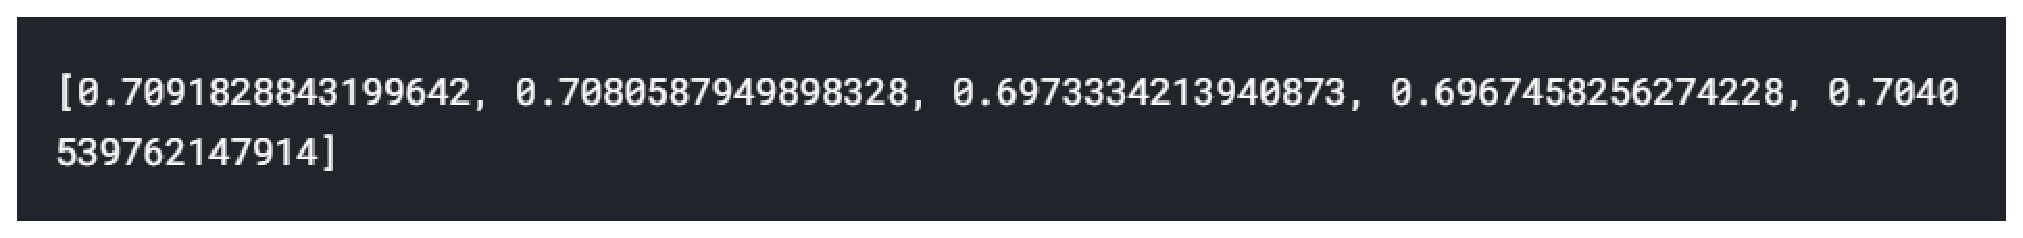
\includegraphics[width=1.0\linewidth,height=.1\linewidth]{C:/FLIP01report/picture/jaccard-BERT.eps}
\end{center}
\end{slide}

%%=========================================================================================
%%=========================================================================================

\begin{slide}[toc=,bm=]{Test Model-BERT}
\begin{table}[tb]
\setlength{\abovecaptionskip}{0pt}
\setlength{\belowcaptionskip}{2pt}
\centering
\caption{There are 10 Random Comparison Results in The Test Results}
\scalebox{0.63}{
\begin{tabular}{c| c c c}
\toprule
%\centering
   & \texttt{textID}  & \texttt{text}  & \texttt{selected_text}\\
\midrule
$0$
&  {$12005b65fc$}	&  {$Waiting for my turn on wii fit gym closed$}	
	&  {$	waiting for my turn on wii fit gym closed$}\\
$1$
&  {$bcf13877f7$}	&  {$Good morning everyone$}	
	&  {$good$}\\
$2$
&  {$575e4a89fe$}	&  {$tts ridiculously sweet of you$}	
	&  {$ridiculously sweet of you$}\\
$3$	
&  {$a0b1828b67$}	&  {$Brides a la mode' pow wow first thing this morning Th...$}	
	&  {$lovely$}\\
$4$
&  {$472c3e2c41$}	&  {$Getting somewhere with my first 'real' KiokuDB and catal...$}	
	&  {$getting somewhere with my first 'real' kiokudb and cata...$}\\
$5$	
&  {$ce71d002ec$}	&  {$Mommas day is may 10th! Don`t forget to do something nice...$}	
	&  {$nice$}\\
$6$
&  {$8db4aaef4a$}	&  {$watching the notebook$}	
	&  {$watching the notebook$}\\
$7$	
&  {$895de1648c$}	&  {$really tired. and have to work the whole day tomorrow, t...$}	
	&  {$really tired.$}\\
$8$
&  {$78d89e7c64$}	&  {$Yeah prbly pickin up songs for SingStar. Haven`t checke...$}	
	&  {$yeah prbly pickin up songs for singstar. haven`t checke...$}\\
$9$	
&  {$756d255e40$}	&  {$is at home with a pukey boy! Poor little baby$}	
	&  {$poor little baby$}\\
\bottomrule
\end{tabular}
}
\end{table}
\end{slide}

\section{Thanks}

\end{document}

\endinput
